% Copyright © 2012 Edward O'Callaghan. All Rights Reserved.
% !Tex root = Real Analysis I.tex

\section{Fourier Transform} % (fold)
\label{sec:fourier}

\begin{defn}[Fourier transform]
	Let $f: \R \to \C$ be an absolutely integrable function
	on $\R$. The $\emph{Fourier transform}$
	$\mathcal{F}(f) \equiv \hat{f}$ of $f$ is defined by the
	integral
	\[
		\hat{f}(\omega) = \frac{1}{\sqrt{2 \pi}}
		\int_{\R} f(x) e^{-i \omega x} \mathrm{d}x .
	\]
\end{defn}

\begin{defn}[Characteristic function]
	\[
		\chi_{(-a,a)}(x) \doteq
		\begin{cases}
			1 & \text{if } |x| < a,\\
			0 & \text{if } |x| \geq a.
		\end{cases}
	\]
\end{defn}

\begin{exmp}
	Suppose $f(x) = \chi_{(-1,1)}(x)$. Find the Fourier
	transform $\hat{f}(\omega)$.

	\begin{align*}
		\hat{f}(\omega) &=
		\frac{1}{\sqrt{2 \pi}} \int_{\R} f(x) e^{-i \omega x} \mathrm{d}x
		\\
		&= \frac{1}{\sqrt{2 \pi}} \int_{-\infty}^{\infty} 
		\chi_{(-1,1)}(x) e^{-i \omega x} \mathrm{d}x
		\\
		&= \frac{1}{\sqrt{2 \pi}} \int_{-1}^{1} e^{-i \omega x} \mathrm{d}x
		\\
		&= \frac{1}{\sqrt{2 \pi}}
		\left\{ \frac{e^{-i \omega x}}{- i \omega} \right\}_{-1}^{1}
		\\
		&= \frac{2}{\sqrt{2 \pi}}
		\left\{ \frac{e^{-i \omega x}}{2 \omega i} \right\}_{1}^{-1}
		\\
		&= \sqrt{\frac{2}{\pi}} \left( \frac{\sin(\omega)}{\omega} \right).
	\end{align*}

	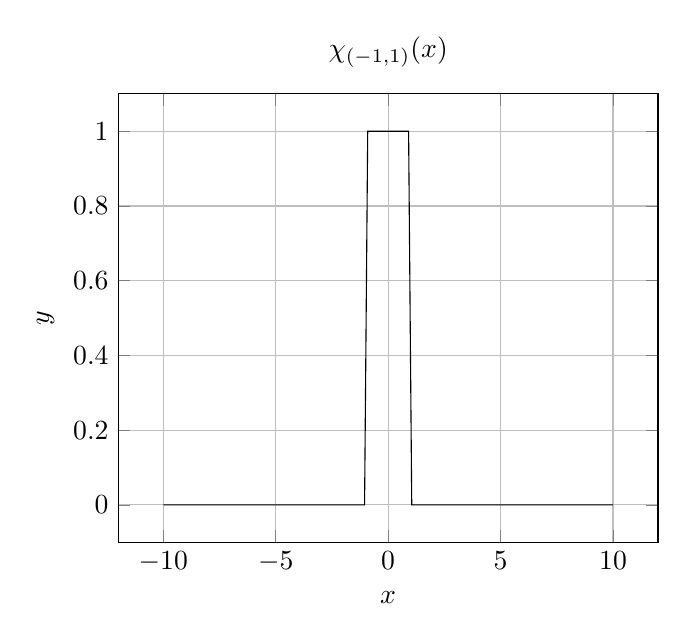
\begin{tikzpicture}
		[declare function={f(\t) = and(\t > -1, \t < 1);}]
		\begin{axis}[domain=-10:10,
			xlabel=$x$,
			ylabel=$y$,
			grid=major,
			title=$\chi_{(-1,1)}(x)$
		]
			\plot[samples=144] (\x,{f(x)});
		\end{axis}
	\end{tikzpicture}
	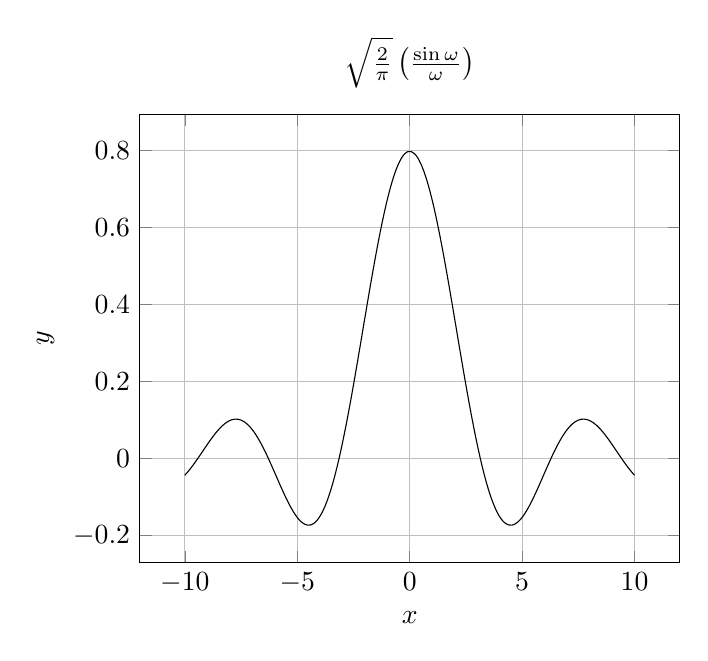
\begin{tikzpicture}
		[declare function={
		g(\t) = ((sqrt(2/pi))*(sin(\t r)/(\t)));
	}]
	\begin{axis}[domain=-10:10,
			xlabel=$x$,
			ylabel=$y$,
			grid=major,
		title=$\sqrt{\frac{2}{\pi}} \left( \frac{\sin{\omega}}{\omega} \right)$]
			\plot[samples=144,smooth] (\x,{g(\x)});
		\end{axis}
	\end{tikzpicture}
\end{exmp}
